\documentclass{article}
\usepackage{a4wide}
\usepackage{norsk}
\usepackage{amsmath}
\usepackage{amssymb}
\usepackage{dsfont}
%\usepackage[dvips]{epsfig}
%\usepackage{graphicx}
\usepackage{fancyhdr}
\usepackage{listings}
\usepackage{nomencl}
\usepackage[pdftex]{graphicx}

\usepackage{float}
\restylefloat{table}

\pagestyle{fancy}
\lhead{\footnotesize \parbox{11cm}{Andreas Johann H\"ormer (753179)}}
\rhead{\footnotesize {Assignment 3}}
\chead{\footnotesize {TET4135}}

\begin{document}
%	\paragraph{Name, Studentnr: }Andreas H\"ormer (753179)
%	\paragraph{Assignment 3}Optimal generation dispatch (Date: 18.02.2014)
	\section*{General}
		\subsection*{power station 1}
			Costs of starting and stoping are assumed negligible ($=0$).
			\begin{itemize}
				\item $K_1=500+45\cdot P_1+0.075\cdot P_1^2 [EUR/h]$
				\item $P_{1_{min}}=20MW$
				\item $P_{1_{max}}=100MW$
			\end{itemize}
		\subsection*{power station 2}
			\begin{itemize}
				\item $K_2=750+52\cdot P_2+0.025\cdot P_2^2 [EUR/h]$
				\item $P_{2_{min}}=40MW$
				\item $P_{2_{max}}=200MW$
			\end{itemize}
	\section{optimal operation of both stations}
		minimum costs, where K1 and K2 intersect ($K_1=K_2$). This is at a production value of $P=169.5MW$

\begin{figure}[htbp]
\begin{center}
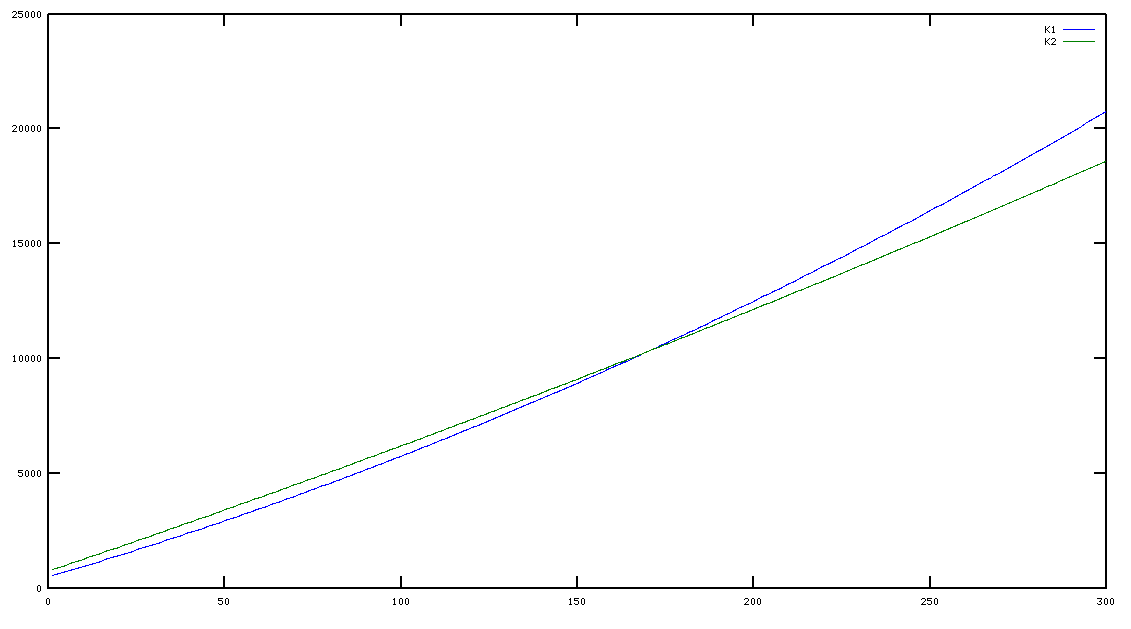
\includegraphics[width=15cm,keepaspectratio=true]{costs}
\caption{costs}
\label{increasing costs for both power stations}
\end{center}
\end{figure}

	\section{Production alternatives}
	\subsection{operation possibilities}
In table \ref{tab:oppos} the possibilities for plant combination at different production intervals is listed.
	\begin{table}[hbt!]
\begin{center}
\begin{tabular}[h]{|c|c|c|c|}
\hline 
Interval (MW)	 & $K_1$ 		& $K_2$ 		& $K_1+K_2$		\\ 
\hline
20..40 			& \checkmark	&	x			& x				\\
40..60 & 			\checkmark & \checkmark  & x				\\
60..100 & 		 \checkmark	& \checkmark	& \checkmark 	\\
100..200 		& x				& \checkmark	& \checkmark	\\
200..300 		& x				& x				& \checkmark	\\
\hline
\end{tabular}
\caption{Operation possibilities for different production}\label{tab:oppos}
\end{center}
\end{table}

\subsection{cost function}
	\begin{equation}
		K_1=500+45\cdot P_1 + 0.075 P_1^2
		\label{f:K1}
	\end{equation}
	\begin{equation}
		K_2=750+52\cdot P_2 + 0.025 P_2^2
		\label{f:K2}
	\end{equation}
The equations \ref{f:K1} and \ref{f:K2} can be derived and the equal marginal costs calculated.
	\begin{equation}
		\frac{dK_1}{dP_1}=45+0.15\cdot P_1
		\label{f:dK1}
	\end{equation}
	\begin{equation}
		\frac{dK_2}{dP_2}=52+0.05\cdot P_2
		\label{f:dK2}
	\end{equation}
	The total costs are minimal where equations \ref{f:dK1} and \ref{f:dK2} are the same. For production of less than 40MW the operation of plant 1 only is possible. So the cost function is not listed seperately.
	\subsubsection{interval 40MW-60MW}
		The Lagrange function can be written as
		\begin{equation}
			L=-(K_1+K_2)+\lambda(P_1+P_2-P_{max})
	 		\label{f:lagrange}
		\end{equation}
In this formulary \ref{f:lagrange} the cost functions for the two generation units can be filled in and the Lagrange function be derived afterwards.
		$$L=-(500+45\cdot P_1+0.075\cdot P_1^2+750+52\cdot P_2+0.025\cdot P_2^2+\lambda(P_1+P_2-60)$$
		$$L=-(1250+45\cdot P_1 + 52\cdot P_2 + 0.075\cdot P_1^2+0.025\cdot P_2^2)+\lambda(P_1+P_2-60)$$
		$$\frac{dL}{dP_1}=-(45+0.15P_1)+\lambda=0$$
		$$\frac{dL}{dP_2}=-(52+0.05P_2)+\lambda=0$$
With this derivates the optimal production amount for $P_1$ and $P_2$ can be calculated.
		$$45+0.15P_1=52+0.05P_2$$
		$$P_1=\frac{1}{3}(P_2+140)$$
	Now the constraint $P_1+P_2=60$ can be filled in.
		$$\frac{1}{3}(P_2+140)+P_2=60$$
		$$P_2=10$$
		This value is the optimum, but it is not ok due to missmatching the constraint. So the production level has to be set to the smallest possible value $P_2$ can procuce for 2-station operation. The production therefore is
		\begin{itemize}
			\item $P_2=P_{2_{min}}=40MW$
			\item $P_1=60MW-40MW=20MW$
		\end{itemize}
		Both values are meeting with the constraints, so this is the optimal solution for two station operation. The costs are calculated as follows:
		\begin{itemize}
			\item $K_1$ only: $K_1(60)=500+45\cdot 60+0.075\cdot 60^2=3470EUR$
			\item $K_2$ only: $K_2(60)=750+52\cdot 60+0.025\cdot 60^2=3960EUR$
			\item $K_1+K_2$: $K=1250+45\cdot 20+0.075\cdot 20^2 + 52\cdot 40+0.025\cdot 40^2=4300EUR$
		\end{itemize}
	\subsubsection{interval 60MW-100MW}
This interval is calculated using tables and increasing the production amount with regard to the actual costs. The calculation steps are listed in table \ref{tab:60100MW}.
	\begin{table}[hbt!]
		\begin{center}
			\begin{tabular}[h]{|r||c|c|c||p{5cm}|}
				\hline 
				($P_1$,$P_2$) [MW] & $\frac{dK_1}{dP_1}$ & $\frac{dK_2}{dP_2}$ & difference & comment\\
				\hline
				\hline
				(0,0)	&	45	&	52	&	$\Delta P_1=+20$	&	costs without production									\\
						&    	&   	& 	$\Delta P_2=+40$ 	&					    										\\
				\hline
				(20,40) &	48	&	54	&	$\Delta P_1=+20$	&	lower production limit, increasing $P_1$ due to lower costs	\\
				\hline
				(40,40) &	51	&	54	&	$\Delta P_1=+20$	&	increase $P_1$, costs are still lower						\\
				\hline
				(60,40) &	54	&	54	&						&	costs are equal, sum of production is 100MW					\\
				\hline
			\end{tabular}
			\caption{Calculation of production amount in interval 60MW-100MW}\label{tab:60100MW}
		\end{center}
	\end{table}
	The costs for the production of 100MW are therefore
		\begin{itemize}
			\item $K_1$ only: $K_1(100)=500+45\cdot 100+0.075\cdot 100^2=5750EUR$
			\item $K_2$ only: $K_2(100)=750+52\cdot 100+0.025\cdot 100^2=6200EUR$
			\item $K_1+K_2$: $K=1250+45\cdot 60+0.075\cdot 60^2 + 52\cdot 40+0.025\cdot 40^2=6340EUR$
		\end{itemize}
	\subsubsection{interval 100MW-200MW}
For the interval from 100MW to 200MW the calculation is also done in a table. The steps are listed in table \ref{tab:100200MW}. Because of the fact, that the calculation principle is always the same, some calculation steps in the middle are not listed.
	\begin{table}[hbt!]
		\begin{center}
			\begin{tabular}[h]{|r||c|c|c||p{5cm}|}
				\hline 
				($P_1$,$P_2$) [MW] & $\frac{dK_1}{dP_1}$ & $\frac{dK_2}{dP_2}$ & difference & comment\\
				\hline
				\hline
				(60,40) &	54		&	54		&	$\Delta P=+10$		&	end point of last calculation, starting point for this one. The costs are equal, so both stations get the same amount of production increase.\\
				\hline
				(70,50) & 	55.5	&	54.5	&	$\Delta P_2=+10$	&	due to cheaper production of $P_2$ increase production of this generation unit\\
				\hline
				(70,60) & 	55.5	&	55		&	$\Delta P_2=+10$	&	$P_2$ still cheaper\\
				\hline
				...		&	...		&	...		&	...					&		...		\\
				\hline
				(80,100)&	57		&	57		&	$\Delta P_1=+3$		&	the amount of power production (200MW) is nearly reached, so decrease the step size\\
						&			&			&	$\Delta P_2=+10$	&	\\
				\hline
				(83,110)&	57.45	&	57.5	&	$\Delta P_1=+1$		&	$P_1$ is not much cheaper, so increase $P_2$ little bit more\\
						&			&			&	$\Delta P_2=+6$		&	\\
				\hline
				(84,116)&	57.6	&	57.8	&	$\Delta P_1=+1$		&	the production amount is reached, but the costs are not equal, so customizing\\
						&			&			&	$\Delta P_2=-1$		&	\\
				\hline
				(85,115)&	57.75 	&	57.75	&						& equal costs\\
				\hline
			\end{tabular}
			\caption{Calculation of production amount in interval 100MW-200MW}\label{tab:100200MW}
		\end{center}
	\end{table}
	As in the table can be seen, the optimal combination for 200MW of produced power is $P_1=85MW$ and $P_2=115MW$. The costs for the two possible generation options are
		\begin{itemize}
			\item $K_2$ only: $K_2(200)=750+52\cdot 200+0.025\cdot 200^2=12750EUR$
			\item $K_1+K_2$: $K=1250+45\cdot 85+0.075\cdot 85^2 + 52\cdot 115+0.025\cdot 115^2=11927.5EUR$
		\end{itemize}
	\subsubsection{interval 200MW-300MW}
In this calculation step the wanted power is in a range, that it is only possible to generate with both generation plants. For 300MW of power both stations have to be utilized full. Thus the costs are
	\begin{itemize}
		\item $K_1+K_2$: $K=1250+45\cdot 100+0.075\cdot 100^2 + 52\cdot 200+0.025\cdot 200^2=17900EUR$
	\end{itemize}
	\subsection{best combination, operation for generation unit 1}
		To get the best generation option the costs are important. Best alternative is that where the costs are lowest.
		\begin{itemize}
			\item 20-40MW:$K_1$ (only possibility)
			\item 40-60MW: $K_1$
			\item 60-100MW: $K_1$
			\item 100-200MW: $K_1+K_2$
			\item 200-300MW: $K_1+K_2$
		\end{itemize}

%Grafik
		
	\section{calculation with emissions}
The maximal allowed emissions are $E_{max}=120t$, the wanted power level 250MW. For calculating the optimal combination of the generation units with respect to the emissions, the Lagrange function has to be modified.
	\begin{itemize}
		\item $K_1$: $e_1=0.55t/MWh$
		\item $K_2$: $e_2=0.45t/MWh$
	\end{itemize}
	\begin{equation}
		L=-(1250+45\cdot P_1+52\cdot P_2+0.075\cdot P_1^2+0.025\cdot P_2^2)+\lambda(P_1+P_2-250)+\mu(120-0.55\cdot P_1-0.45\cdot P_2)
		\label{f:lagrangeadvanced}
	\end{equation}
	This modified Lagrange function in equation \ref{f:lagrangeadvanced} can now be derived. 
	$$\frac{dL}{dP_1}=-45+\lambda-0.55\cdot\mu$$
	$$\frac{dL}{dP_2}=-52+\lambda-0.45\cdot\mu$$
	With respect to the constraints the new values for the production values of $P_1$ and $P_2$ can be calculated.
	$$0.55\cdot P_1+0.45\cdot P_2\leq 120$$
	$$0.55(250-P_2)+0.45\cdot P_2\leq 120$$
	$$-0.1\cdot P_2\leq -17.5$$
	$$P_2\geq 175$$
	Thus the production values are
	\begin{itemize}
		\item $P_1=75MW$
		\item $P_2=175MW$
	\end{itemize}
The production amounts are modified in that way, that the production plant is penalized by the emission constraint. Production amounts are moving to $K_2$ so that $K_2$ is now producing more power than without the emission term.
\end{document}
